\documentclass[8pt,aspectratio=169]{beamer}
\usetheme{Madrid}
\usepackage{graphicx}
\usepackage{booktabs}
\usepackage{adjustbox}
\usepackage{multicol}
\usepackage{amsmath}

% Color definitions
\definecolor{mlblue}{RGB}{0,102,204}
\definecolor{mlpurple}{RGB}{51,51,178}
\definecolor{mllavender}{RGB}{173,173,224}
\definecolor{mllavender2}{RGB}{193,193,232}
\definecolor{mllavender3}{RGB}{204,204,235}
\definecolor{mllavender4}{RGB}{214,214,239}
\definecolor{mlorange}{RGB}{255, 127, 14}
\definecolor{mlgreen}{RGB}{44, 160, 44}
\definecolor{mlred}{RGB}{214, 39, 40}
\definecolor{mlgray}{RGB}{127, 127, 127}
\definecolor{lightgray}{RGB}{240, 240, 240}
\definecolor{midgray}{RGB}{180, 180, 180}

% Theme colors
\setbeamercolor{palette primary}{bg=mllavender3,fg=mlpurple}
\setbeamercolor{palette secondary}{bg=mllavender2,fg=mlpurple}
\setbeamercolor{palette tertiary}{bg=mllavender,fg=white}
\setbeamercolor{palette quaternary}{bg=mlpurple,fg=white}
\setbeamercolor{structure}{fg=mlpurple}
\setbeamercolor{section in toc}{fg=mlpurple}
\setbeamercolor{subsection in toc}{fg=mlblue}
\setbeamercolor{title}{fg=mlpurple}
\setbeamercolor{frametitle}{fg=mlpurple,bg=mllavender3}
\setbeamercolor{block title}{bg=mllavender2,fg=mlpurple}
\setbeamercolor{block body}{bg=mllavender4,fg=black}

\setbeamertemplate{navigation symbols}{}
\setbeamertemplate{itemize items}[circle]
\setbeamertemplate{enumerate items}[default]
\setbeamersize{text margin left=5mm,text margin right=5mm}

\newcommand{\bottomnote}[1]{%
\vfill
\vspace{-2mm}
\textcolor{mllavender2}{\rule{\textwidth}{0.4pt}}
\vspace{1mm}
\footnotesize
\textbf{#1}
}

% === Additional packages for mini-lecture ===
\usepackage{tikz}
\usepackage{pgfplots}
\pgfplotsset{compat=1.18}
\usetikzlibrary{arrows.meta, positioning, shapes.geometric, decorations.pathreplacing}

% === Mini-lecture accent colors (skill-documented values) ===
\definecolor{dfteal}{RGB}{0, 153, 153}
\definecolor{dfred}{RGB}{204, 51, 51}

% === Exampleblock styling ===
\setbeamercolor{exampleblock title}{bg=dfteal!20,fg=dfteal!80!black}
\setbeamercolor{exampleblock body}{bg=dfteal!5,fg=black}

% === Compact list command (MUST be defined before any usage) ===
\newcommand{\compactlist}{\setlength{\itemsep}{1pt}\setlength{\parskip}{0pt}\setlength{\parsep}{0pt}}

\title{Market Microstructure in Digital Finance}
\subtitle{When you trade, who sets the price---and who profits?}
\author{Economics of Digital Finance}
\institute{BSc Course}
\date{}

\begin{document}
\begin{frame}[plain]
\titlepage
\end{frame}

% ============================================================
% SLIDE 1: WHY -- What happens when there is no middleman?
% Visual: TikZ comic (dfteal dilemma) RIGHT, text LEFT
% ============================================================
\begin{frame}[t]{What happens when there is no middleman to set the price?}
\begin{columns}[T]
\begin{column}{0.55\textwidth}
\small
In traditional markets, a buyer walks up to a trading floor and a specialist
(a designated person whose job is to match buyers with sellers) sets the price.
But what if there is no specialist, no floor, no human at all---just a
mathematical formula running on a network of computers?

\vspace{2mm}
\footnotesize
\begin{itemize}\compactlist
\item Traditional markets: human intermediaries match orders
      (a buy request paired with a sell request)
\item A new approach: replace all intermediaries with a single equation
\item The equation always gives you a price---but is it a fair one?
\end{itemize}
\end{column}
\begin{column}{0.42\textwidth}
\centering
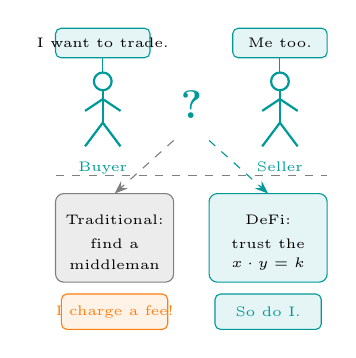
\begin{tikzpicture}[scale=0.75, every node/.style={font=\tiny}]
  % Buyer stick figure
  \draw[dfteal, thick] (0.8,6.2) circle (0.15);
  \draw[dfteal, thick] (0.8,6.05) -- (0.8,5.5);
  \draw[dfteal, thick] (0.8,5.9) -- (0.5,5.7);
  \draw[dfteal, thick] (0.8,5.9) -- (1.1,5.7);
  \draw[dfteal, thick] (0.8,5.5) -- (0.5,5.1);
  \draw[dfteal, thick] (0.8,5.5) -- (1.1,5.1);
  \node[below, dfteal] at (0.8,5.0) {Buyer};

  % Buyer speech bubble
  \draw[dfteal, rounded corners=2pt, fill=dfteal!10]
    (0.0,6.6) rectangle (1.6,7.1);
  \node at (0.8,6.85) {I want to trade.};
  \draw[dfteal] (0.8,6.6) -- (0.8,6.35);

  % Seller stick figure
  \draw[dfteal, thick] (3.8,6.2) circle (0.15);
  \draw[dfteal, thick] (3.8,6.05) -- (3.8,5.5);
  \draw[dfteal, thick] (3.8,5.9) -- (3.5,5.7);
  \draw[dfteal, thick] (3.8,5.9) -- (4.1,5.7);
  \draw[dfteal, thick] (3.8,5.5) -- (3.5,5.1);
  \draw[dfteal, thick] (3.8,5.5) -- (4.1,5.1);
  \node[below, dfteal] at (3.8,5.0) {Seller};

  % Seller speech bubble
  \draw[dfteal, rounded corners=2pt, fill=dfteal!10]
    (3.0,6.6) rectangle (4.6,7.1);
  \node at (3.8,6.85) {Me too.};
  \draw[dfteal] (3.8,6.6) -- (3.8,6.35);

  % Central question mark
  \node[font=\Large\bfseries, dfteal] at (2.3,5.8) {?};

  % Dividing line
  \draw[mlgray, dashed] (0,4.6) -- (4.6,4.6);

  % Left path: traditional
  \draw[mlgray, rounded corners=3pt, fill=mlgray!15]
    (0.0,2.8) rectangle (2.0,4.3);
  \node[align=center] at (1.0,3.85) {Traditional:};
  \node[align=center] at (1.0,3.45) {find a};
  \node[align=center] at (1.0,3.1) {middleman};
  % Middleman speech bubble
  \draw[mlorange, rounded corners=2pt, fill=mlorange!10]
    (0.1,2.0) rectangle (1.9,2.6);
  \node[mlorange] at (1.0,2.3) {I charge a fee!};

  % Right path: DeFi
  \draw[dfteal, rounded corners=3pt, fill=dfteal!10]
    (2.6,2.8) rectangle (4.6,4.3);
  \node[align=center] at (3.6,3.85) {DeFi:};
  \node[align=center] at (3.6,3.45) {trust the};
  \node[align=center, font=\tiny\itshape] at (3.6,3.1) {$x \cdot y = k$};
  % Formula speech bubble
  \draw[dfteal, rounded corners=2pt, fill=dfteal!10]
    (2.7,2.0) rectangle (4.5,2.6);
  \node[dfteal] at (3.6,2.3) {So do I.};

  % Dashed arrows from question mark to paths
  \draw[dashed, ->, >=Stealth, mlgray] (2.0,5.2) -- (1.0,4.3);
  \draw[dashed, ->, >=Stealth, dfteal] (2.6,5.2) -- (3.6,4.3);
\end{tikzpicture}
\end{column}
\end{columns}

\begin{block}{Key Insight}
Both systems solve the same problem---connecting buyers with sellers---but they
make fundamentally different trade-offs between human judgment and mathematical certainty.
\end{block}

\bottomnote{Market microstructure (the study of how trading mechanisms work at a detailed level)
explains why these design choices matter for every trader.}
\end{frame}

% ============================================================
% SLIDE 2: FEEL -- Have you ever been the last one to know?
% Visual: Full-width text-only with exampleblock
% ============================================================
\begin{frame}[t]{Have you ever been the last one to know?}
\small
Imagine you are at an auction. You bid on an item, feeling confident about your price.
But someone in the room already knows what the item will sell for tomorrow---and they
quietly outbid you by just enough to win. You only find out later that the price was
never really fair to begin with.

\vspace{3mm}
\footnotesize
\textit{Think about a time you made a purchase and later realized someone else had better
information. How did that affect the price you paid?}

\vspace{3mm}
\footnotesize
This feeling---of trading against someone with an advantage---is the core problem
of market microstructure. When some participants know more than others, prices become
skewed. The technical term is information asymmetry (when one side of a transaction
knows more than the other). Understanding who knows what, and when, is the key to
understanding why some trading systems are fairer than others.

\begin{exampleblock}{Reflection}
Every market mechanism is ultimately a response to the same question: how do you set
a fair price when participants have unequal information?
\end{exampleblock}

\bottomnote{Information asymmetry shapes every trading mechanism ever designed,
from ancient bazaars to modern algorithms.}
\end{frame}

% ============================================================
% SLIDE 3: WHAT -- How do the two architectures differ?
% Visual: Comparison table LEFT, text RIGHT
% ============================================================
\begin{frame}[t]{How do the two trading architectures actually differ?}
\begin{columns}[T]
\begin{column}{0.55\textwidth}
\small
Two dominant architectures exist for matching trades. An order book (a list of all
pending buy and sell orders, ranked by price) relies on participants actively posting
offers. An automated market maker, or AMM (a smart contract---self-executing code on a
blockchain---that uses a formula to set prices), replaces human market makers entirely.

\vspace{1mm}
\begin{adjustbox}{max width=\linewidth}
\scriptsize
\begin{tabular}{lll}
\toprule
\textbf{Dimension} & \textbf{Order Book} & \textbf{AMM} \\
\midrule
\shortstack[l]{Price\\setter} & \shortstack[l]{Traders posting\\orders} & \shortstack[l]{Mathematical\\formula} \\[2pt]
\shortstack[l]{Liquidity\\source} & \shortstack[l]{Professional\\market makers} & \shortstack[l]{Anyone who\\deposits tokens} \\[2pt]
Execution & \shortstack[l]{Match buy\\with sell} & \shortstack[l]{Trade against a pool\\(shared token reserve)} \\[2pt]
Transparency & \shortstack[l]{Partial (some\\orders hidden)} & \shortstack[l]{Full (formula\\is public code)} \\[2pt]
\shortstack[l]{Capital\\need} & Active management & Passive deposit \\[2pt]
Vulnerability & \shortstack[l]{Spoofing\\(fake orders)} & \shortstack[l]{Value extraction\\by bots} \\
\bottomrule
\end{tabular}
\end{adjustbox}
\end{column}
\begin{column}{0.42\textwidth}
\footnotesize
Key difference: an order book is a \textit{negotiation}---prices emerge from
competing offers. An AMM is a \textit{computation}---the price is whatever the
formula says, with no negotiation.

\vspace{2mm}
\footnotesize
Each architecture has a different failure mode: order books fail when market makers
withdraw (liquidity vanishes), while AMMs always have liquidity but the price may
be stale (outdated relative to other markets).
\end{column}
\end{columns}

\begin{block}{Key Insight}
Order books let the market negotiate prices; automated market makers let mathematics
dictate them---neither approach is strictly superior.
\end{block}

\bottomnote{The choice of trading architecture determines who bears risk, who earns fees,
and how quickly prices reflect new information.}
\end{frame}

% ============================================================
% SLIDE 4: CASE -- What happens inside the formula?
% Visual: TikZ step diagram LEFT, narration RIGHT
% ============================================================
\begin{frame}[t]{What happens inside the formula when you press swap?}
\begin{columns}[T]
\begin{column}{0.55\textwidth}
\centering
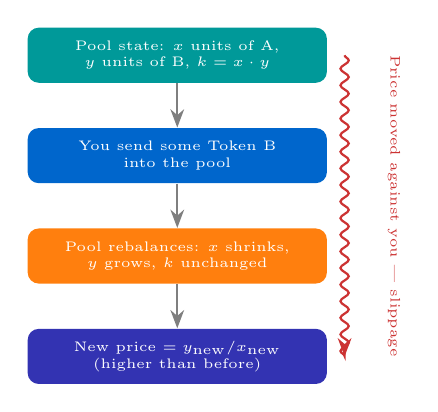
\begin{tikzpicture}[scale=0.85, every node/.style={font=\tiny},
  box/.style={rounded corners=4pt, minimum width=3.8cm, minimum height=0.7cm,
              align=center, text=white, font=\tiny}]
  % Box 1
  \node[box, fill=dfteal] (b1) at (0,5.5)
    {Pool state: $x$ units of A,\\$y$ units of B, $k = x \cdot y$};
  % Box 2
  \node[box, fill=mlblue] (b2) at (0,4.0)
    {You send some Token B\\into the pool};
  % Box 3
  \node[box, fill=mlorange] (b3) at (0,2.5)
    {Pool rebalances: $x$ shrinks,\\$y$ grows, $k$ unchanged};
  % Box 4
  \node[box, fill=mlpurple] (b4) at (0,1.0)
    {New price $= y_{\text{new}} / x_{\text{new}}$\\(higher than before)};

  % Arrows between boxes
  \draw[->, >=Stealth, thick, mlgray] (b1) -- (b2);
  \draw[->, >=Stealth, thick, mlgray] (b2) -- (b3);
  \draw[->, >=Stealth, thick, mlgray] (b3) -- (b4);

  % Slippage arrow on right side
  \draw[->, >=Stealth, thick, dfred, decorate,
    decoration={snake, amplitude=1.5pt, segment length=6pt}]
    (2.5,5.5) -- (2.5,1.0);
  \node[rotate=-90, dfred, font=\tiny, anchor=south] at (3.0,3.25)
    {Price moved against you --- slippage};
\end{tikzpicture}
\end{column}
\begin{column}{0.42\textwidth}
\small
The most common AMM formula is the constant product rule:
$x \cdot y = k$, where $x$ and $y$ are the quantities of two tokens
in a shared pool, and $k$ is a constant that never changes.
The price at any moment is simply $y / x$.

\vspace{2mm}
\footnotesize
\begin{enumerate}\compactlist
\item \textbf{Before the trade:} Pool holds $x$ units of Token A
  and $y$ units of Token B. Product: $x \cdot y = k$.
\item \textbf{You buy Token A:} You send some Token B into the pool.
  Token B reserve grows; Token A reserve shrinks---but $k$ stays the same.
\item \textbf{New price:} Because there is now less Token A and more
  Token B, the ratio $y/x$ rises. Token A is more expensive.
\item \textbf{Slippage} (the gap between expected and actual price):
  The bigger your trade relative to the pool, the more the price moves
  against you.
\end{enumerate}
\end{column}
\end{columns}

\begin{block}{Key Insight}
The constant product formula guarantees a price for any trade size, but larger trades
pay progressively worse prices---the pool protects itself by making big trades expensive.
\end{block}

\bottomnote{Slippage is not a bug---it is the mechanism by which the formula discourages
trades that would drain the pool.}
\end{frame}

% ============================================================
% SLIDE 5: HOW -- How does each system keep prices honest?
% Visual: TikZ architecture diagram RIGHT, text LEFT
% ============================================================
\begin{frame}[t]{How does each system keep prices honest?}
\begin{columns}[T]
\begin{column}{0.55\textwidth}
\small
\textbf{Order Book Architecture}

\footnotesize
\begin{itemize}\compactlist
\item \textbf{Price discovery} (the process by which markets determine
  the correct price): Traders submit limit orders (offers to buy or
  sell at a specific price) that reveal their valuation
\item \textbf{Correction mechanism:} If the price drifts, arbitrageurs
  (traders who profit by exploiting price differences between markets)
  buy cheap and sell expensive, pushing the price back
\item \textbf{Speed advantage:} Professional firms with fast computers
  react to new information in milliseconds
\item \textbf{Weakness:} If professionals withdraw, the book empties
  and prices become unreliable
\end{itemize}

\vspace{1mm}
\small
\textbf{AMM Architecture}

\scriptsize
\begin{itemize}\compactlist
\item \textbf{Price discovery:} The formula sets a price, but it only
  updates when someone trades---it cannot react to external news on its own
\item \textbf{Correction:} Arbitrageurs compare AMM price
  to other markets and trade until they match
\item \textbf{Always-on liquidity:} The formula never refuses a trade,
  but the price may lag behind reality
\item \textbf{Weakness:} The gap between AMM price and true
  price is profit for arbitrageurs---a cost to liquidity providers
\end{itemize}
\end{column}
\begin{column}{0.42\textwidth}
\centering
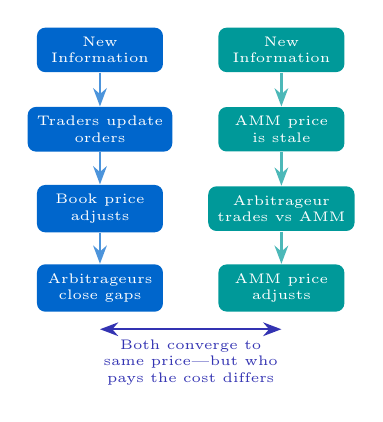
\begin{tikzpicture}[scale=0.72, every node/.style={font=\tiny},
  sbox/.style={rounded corners=3pt, minimum width=1.6cm, minimum height=0.55cm,
               align=center, font=\tiny, text=white}]
  % LEFT stack: Order Book
  \node[sbox, fill=mlblue] (ob1) at (0,6.0) {New\\Information};
  \node[sbox, fill=mlblue] (ob2) at (0,4.6) {Traders update\\orders};
  \node[sbox, fill=mlblue] (ob3) at (0,3.2) {Book price\\adjusts};
  \node[sbox, fill=mlblue] (ob4) at (0,1.8) {Arbitrageurs\\close gaps};

  \draw[->, >=Stealth, thick, mlblue!70] (ob1) -- (ob2);
  \draw[->, >=Stealth, thick, mlblue!70] (ob2) -- (ob3);
  \draw[->, >=Stealth, thick, mlblue!70] (ob3) -- (ob4);

  % RIGHT stack: AMM
  \node[sbox, fill=dfteal] (am1) at (3.2,6.0) {New\\Information};
  \node[sbox, fill=dfteal] (am2) at (3.2,4.6) {AMM price\\is stale};
  \node[sbox, fill=dfteal] (am3) at (3.2,3.2) {Arbitrageur\\trades vs AMM};
  \node[sbox, fill=dfteal] (am4) at (3.2,1.8) {AMM price\\adjusts};

  \draw[->, >=Stealth, thick, dfteal!70] (am1) -- (am2);
  \draw[->, >=Stealth, thick, dfteal!70] (am2) -- (am3);
  \draw[->, >=Stealth, thick, dfteal!70] (am3) -- (am4);

  % Bottom double arrow
  \draw[<->, >=Stealth, thick, mlpurple] (ob4.south) ++(0,-0.3)
    -- ++(3.2,0) node[midway, below, align=center, font=\tiny, text=mlpurple]
    {Both converge to\\same price---but who\\pays the cost differs};
\end{tikzpicture}
\end{column}
\end{columns}

\begin{block}{Key Insight}
Order books react to information through human decisions; AMMs react through
arbitrage trades---both reach the same price, but the cost falls on different participants.
\end{block}

\bottomnote{Price discovery is never free---the question is whether the cost falls
on professional market makers or passive liquidity providers.}
\end{frame}

% ============================================================
% SLIDE 6: RISK -- What if someone can see your trade?
% Visual: TikZ comic (dfred failure) RIGHT, text LEFT
% ============================================================
\begin{frame}[t]{What if someone can see your trade before it happens?}
\begin{columns}[T]
\begin{column}{0.55\textwidth}
\footnotesize
On a blockchain, pending transactions sit in a public waiting area
(the mempool---a queue of unconfirmed transactions visible to everyone).
A bot (an automated program) can see your trade and insert its own trades
around yours---before your transaction is confirmed.

\vspace{1mm}
\footnotesize
\begin{itemize}\compactlist
\item \textbf{Step 1---Front-run:} The bot buys the token you want,
  pushing the price up
\item \textbf{Step 2---Your trade:} You buy at the inflated price,
  pushing it up further
\item \textbf{Step 3---Back-run:} The bot sells at the higher price,
  pocketing the difference
\item \textbf{Result:} You paid more than you should have; the bot
  extracted the difference as profit
\end{itemize}

\vspace{1mm}
\scriptsize
This is a \textbf{sandwich attack} (a front-run and back-run
wrapped around a victim's trade), a form of \textbf{MEV} (maximal
extractable value---profit from reordering or inserting transactions).
\end{column}
\begin{column}{0.42\textwidth}
\centering
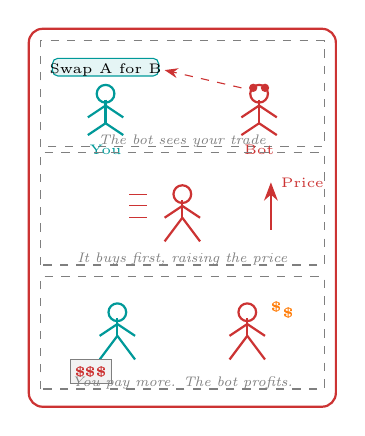
\begin{tikzpicture}[scale=0.75, every node/.style={font=\tiny}]
  % Border
  \draw[dfred, rounded corners=5pt, thick] (-0.3,-0.2) rectangle (4.9,6.2);

  % PANEL 1: Bot sees your trade
  \draw[mlgray, dashed] (-0.1,4.2) rectangle (4.7,6.0);
  % You stick figure
  \draw[dfteal, thick] (1.0,5.1) circle (0.15);
  \draw[dfteal, thick] (1.0,5.0) -- (1.0,4.6);
  \draw[dfteal, thick] (1.0,4.9) -- (0.7,4.7);
  \draw[dfteal, thick] (1.0,4.9) -- (1.3,4.7);
  \draw[dfteal, thick] (1.0,4.6) -- (0.7,4.4);
  \draw[dfteal, thick] (1.0,4.6) -- (1.3,4.4);
  \node[below, dfteal] at (1.0,4.4) {You};
  % You speech bubble
  \draw[dfteal, rounded corners=2pt, fill=dfteal!10]
    (0.1,5.4) rectangle (1.9,5.7);
  \node at (1.0,5.5) {Swap A for B};

  % Bot figure (angular)
  \draw[dfred, thick] (3.6,5.1) circle (0.15);
  \draw[dfred, thick] (3.6,5.0) -- (3.6,4.6);
  \draw[dfred, thick] (3.6,4.9) -- (3.3,4.7);
  \draw[dfred, thick] (3.6,4.9) -- (3.9,4.7);
  \draw[dfred, thick] (3.6,4.6) -- (3.3,4.4);
  \draw[dfred, thick] (3.6,4.6) -- (3.9,4.4);
  % Binocular eyes
  \draw[dfred, fill=dfred] (3.5,5.2) circle (0.06);
  \draw[dfred, fill=dfred] (3.7,5.2) circle (0.06);
  \node[below, dfred] at (3.6,4.4) {Bot};
  % Peek line
  \draw[dfred, dashed, ->, >=Stealth] (3.3,5.2) -- (2.0,5.5);

  \node[mlgray, font=\tiny\itshape] at (2.3,4.3) {The bot sees your trade};

  % PANEL 2: Bot buys first
  \draw[mlgray, dashed] (-0.1,2.2) rectangle (4.7,4.1);
  % Bot jumping ahead
  \draw[dfred, thick] (2.3,3.4) circle (0.15);
  \draw[dfred, thick] (2.3,3.3) -- (2.3,3.0);
  \draw[dfred, thick] (2.3,3.2) -- (2.0,3.0);
  \draw[dfred, thick] (2.3,3.2) -- (2.6,3.0);
  \draw[dfred, thick] (2.3,3.0) -- (2.0,2.6);
  \draw[dfred, thick] (2.3,3.0) -- (2.6,2.6);
  % Motion lines
  \draw[dfred] (1.7,3.4) -- (1.4,3.4);
  \draw[dfred] (1.7,3.2) -- (1.4,3.2);
  \draw[dfred] (1.7,3.0) -- (1.4,3.0);
  % Price arrow up
  \draw[->, >=Stealth, thick, dfred] (3.8,2.8) -- (3.8,3.6)
    node[right, font=\tiny] {Price};

  \node[mlgray, font=\tiny\itshape] at (2.3,2.3) {It buys first, raising the price};

  % PANEL 3: You pay more, bot profits
  \draw[mlgray, dashed] (-0.1,0.1) rectangle (4.7,2.0);
  % You dismayed
  \draw[dfteal, thick] (1.2,1.4) circle (0.15);
  \draw[dfteal, thick] (1.2,1.3) -- (1.2,1.0);
  \draw[dfteal, thick] (1.2,1.2) -- (0.9,1.0);
  \draw[dfteal, thick] (1.2,1.2) -- (1.5,1.0);
  \draw[dfteal, thick] (1.2,1.0) -- (0.9,0.6);
  \draw[dfteal, thick] (1.2,1.0) -- (1.5,0.6);
  % Receipt
  \draw[mlgray, fill=mlgray!10] (0.4,0.2) rectangle (1.1,0.6);
  \node[dfred, font=\tiny\bfseries] at (0.75,0.4) {\$\$\$};

  % Bot with profit
  \draw[dfred, thick] (3.4,1.4) circle (0.15);
  \draw[dfred, thick] (3.4,1.3) -- (3.4,1.0);
  \draw[dfred, thick] (3.4,1.2) -- (3.1,1.0);
  \draw[dfred, thick] (3.4,1.2) -- (3.7,1.0);
  \draw[dfred, thick] (3.4,1.0) -- (3.1,0.6);
  \draw[dfred, thick] (3.4,1.0) -- (3.7,0.6);
  % Coins
  \node[mlorange, font=\tiny\bfseries] at (3.9,1.5) {\$};
  \node[mlorange, font=\tiny\bfseries] at (4.1,1.4) {\$};

  \node[mlgray, font=\tiny\itshape] at (2.3,0.2) {You pay more. The bot profits.};
\end{tikzpicture}
\end{column}
\end{columns}

\begin{block}{Key Insight}
Transaction transparency---normally a virtue---becomes a vulnerability when others can act on your intentions before you can.
\end{block}

\bottomnote{Maximal extractable value turns the public nature of blockchain transactions into a systematic cost for ordinary traders.}
\end{frame}

% ============================================================
% SLIDE 7: WHERE -- Where does the price actually come from?
% Visual: pgfplots bar chart LEFT, text RIGHT
% ============================================================
\begin{frame}[t]{Where does the price actually come from?}
\begin{columns}[T]
\begin{column}{0.55\textwidth}
\centering
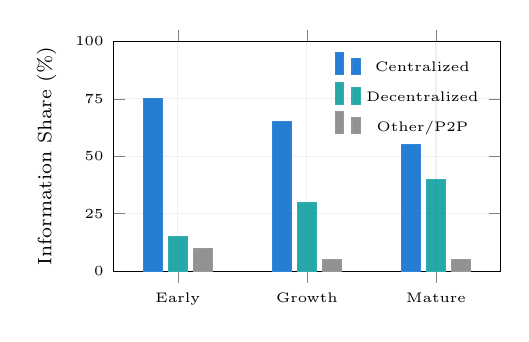
\begin{tikzpicture}
\begin{axis}[
  width=6.5cm,
  height=4.5cm,
  ybar,
  bar width=7pt,
  ymin=0, ymax=100,
  ytick={0,25,50,75,100},
  ylabel={\scriptsize Information Share (\%)},
  ylabel style={font=\scriptsize},
  symbolic x coords={Early,Growth,Mature},
  xtick=data,
  xticklabel style={font=\tiny},
  yticklabel style={font=\tiny},
  legend style={font=\tiny, at={(0.98,0.98)}, anchor=north east,
    legend columns=1, draw=none, fill=none},
  grid=major,
  grid style={lightgray, thin},
  enlarge x limits=0.25,
  every axis plot/.append style={fill opacity=0.85},
]
\addplot[fill=mlblue, draw=mlblue!80] coordinates
  {(Early,75) (Growth,65) (Mature,55)};
\addplot[fill=dfteal, draw=dfteal!80] coordinates
  {(Early,15) (Growth,30) (Mature,40)};
\addplot[fill=mlgray, draw=mlgray!80] coordinates
  {(Early,10) (Growth,5) (Mature,5)};
\legend{Centralized, Decentralized, Other/P2P}
\end{axis}
\end{tikzpicture}
\end{column}
\begin{column}{0.42\textwidth}
\small
When the same asset trades on multiple venues (different exchanges or pools),
which venue sets the ``real'' price? Researchers measure this using
information share (the proportion of price discovery---finding the true
price---contributed by each venue).

\vspace{2mm}
\footnotesize
\begin{itemize}\compactlist
\item Centralized venues tend to lead price discovery because professional
  traders with fast connections concentrate there
\item Decentralized venues tend to follow, adjusting through arbitrage
  with a lag
\item The gap between venues represents a cost: someone profits from
  closing it
\item As decentralized infrastructure matures, the balance may shift
\end{itemize}
\end{column}
\end{columns}

\begin{block}{Key Insight}
Price discovery is not a property of any single venue---it is distributed across
all markets, with the balance shifting as infrastructure and participation evolve.
\end{block}

\bottomnote{Information share measures where new price information first appears;
it shifts over time as market structures mature.}
\end{frame}

% ============================================================
% SLIDE 8: IMPACT -- Who profits and who pays?
% Visual: TikZ stakeholder map LEFT, text RIGHT
% ============================================================
\begin{frame}[t]{Who profits and who pays in each architecture?}
\begin{columns}[T]
\begin{column}{0.55\textwidth}
\centering
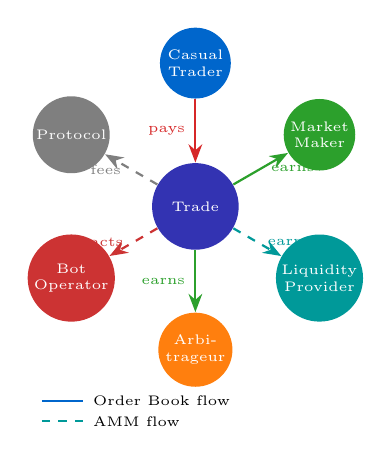
\begin{tikzpicture}[scale=0.65, every node/.style={font=\tiny},
  sat/.style={circle, minimum size=0.9cm, align=center, font=\tiny,
              text=white, inner sep=1pt}]
  % Central node
  \node[sat, fill=mlpurple, minimum size=1.1cm] (center) at (0,0) {Trade};

  % Satellite nodes at roughly 60-degree intervals
  \node[sat, fill=mlblue] (ct) at (90:2.8) {Casual\\Trader};
  \node[sat, fill=mlgreen] (mm) at (30:2.8) {Market\\Maker};
  \node[sat, fill=dfteal] (lp) at (330:2.8) {Liquidity\\Provider};
  \node[sat, fill=mlorange] (arb) at (270:2.8) {Arbi-\\trageur};
  \node[sat, fill=dfred] (bot) at (210:2.8) {Bot\\Operator};
  \node[sat, fill=mlgray] (proto) at (150:2.8) {Protocol};

  % Order book flows (solid)
  \draw[->, >=Stealth, thick, mlred] (ct) -- (center)
    node[midway, left, font=\tiny, text=mlred] {pays};
  \draw[->, >=Stealth, thick, mlgreen] (center) -- (mm)
    node[midway, right, font=\tiny, text=mlgreen] {earns};
  \draw[->, >=Stealth, thick, mlgreen] (center) -- (arb)
    node[midway, left, font=\tiny, text=mlgreen] {earns};

  % AMM flows (dashed)
  \draw[->, >=Stealth, thick, dashed, dfteal] (center) -- (lp)
    node[midway, right, font=\tiny, text=dfteal] {earns};
  \draw[->, >=Stealth, thick, dashed, dfred] (center) -- (bot)
    node[midway, left, font=\tiny, text=dfred] {extracts};
  \draw[->, >=Stealth, thick, dashed, mlgray] (center) -- (proto)
    node[midway, left, font=\tiny, text=mlgray] {fees};

  % Legend
  \draw[thick, mlblue] (-3.0,-3.8) -- (-2.2,-3.8)
    node[right, font=\tiny, text=black] {Order Book flow};
  \draw[thick, dashed, dfteal] (-3.0,-4.2) -- (-2.2,-4.2)
    node[right, font=\tiny, text=black] {AMM flow};
\end{tikzpicture}
\end{column}
\begin{column}{0.42\textwidth}
\small
Every trading architecture creates winners and losers. The same person can be
a winner in one system and a loser in another. Understanding who bears the costs
is essential for evaluating whether a system is fair.

\vspace{2mm}
\footnotesize
\begin{itemize}\compactlist
\item \textbf{Casual traders:} Pay spreads in order books; pay slippage
  plus MEV in AMMs
\item \textbf{Professional market makers:} Earn spreads in order books;
  have no role in AMMs
\item \textbf{Liquidity providers} (depositors): Earn fees but suffer
  impermanent loss (a loss when the price ratio of deposited tokens
  changes) in AMMs
\item \textbf{Arbitrageurs:} Profit from price discrepancies in both
\item \textbf{Bot operators:} Extract MEV from AMMs; limited role in
  order books (front-running is regulated)
\item \textbf{Protocol operators:} Earn listing fees or protocol fees
\end{itemize}
\end{column}
\end{columns}

\begin{block}{Key Insight}
Automated market makers do not eliminate intermediaries---they replace professional
market makers with passive depositors and shift extraction from regulated spreads
to unregulated bot profits.
\end{block}

\bottomnote{No trading architecture is neutral---each embeds a different answer
to the question of who should bear the cost of providing liquidity.}
\end{frame}

% ============================================================
% SLIDE 9: SO WHAT -- Three questions to evaluate any mechanism
% Visual: TikZ triple-balance metaphor RIGHT, text LEFT
% ============================================================
\begin{frame}[t]{Three questions to evaluate any trading mechanism}
\begin{columns}[T]
\begin{column}{0.55\textwidth}
\small
Whether you are a regulator, a developer, or a trader, you can evaluate
ANY trading mechanism---past, present, or future---by asking three questions:

\vspace{2mm}
\footnotesize
\begin{enumerate}\compactlist
\item \textbf{Who sets the price, and how fast does it update?}
  (Measures price discovery quality: faster and more independent sources
  produce better prices)
\item \textbf{Where does liquidity come from, and what does it cost the
  provider?} (Measures sustainability: if providers lose money, liquidity
  will eventually dry up)
\item \textbf{Who can extract value, and is that extraction visible?}
  (Measures fairness: hidden extraction is more dangerous than visible fees)
\end{enumerate}

\vspace{2mm}
\footnotesize
Apply these three questions to any system. A good mechanism scores well on
all three; most real systems trade off one dimension against another. There
is no perfect architecture---only informed choices.
\end{column}
\begin{column}{0.42\textwidth}
\centering
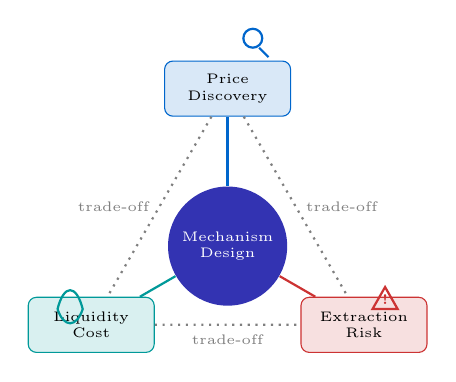
\begin{tikzpicture}[scale=0.8, every node/.style={font=\tiny}]
  % Central pivot
  \node[circle, fill=mlpurple, text=white, minimum size=0.9cm,
        font=\tiny, align=center] (pivot) at (0,0) {Mechanism\\Design};

  % Three arms at 120-degree angles
  % Top: Price Discovery
  \node[rounded corners=3pt, fill=mlblue!15, draw=mlblue,
        minimum width=1.6cm, minimum height=0.7cm, align=center]
    (pd) at (90:2.5) {Price\\Discovery};
  \draw[thick, mlblue] (pivot) -- (pd);
  % Magnifying glass icon
  \draw[mlblue, thick] (0.4,3.3) circle (0.15);
  \draw[mlblue, thick] (0.5,3.15) -- (0.65,3.0);

  % Bottom-left: Liquidity Cost
  \node[rounded corners=3pt, fill=dfteal!15, draw=dfteal,
        minimum width=1.6cm, minimum height=0.7cm, align=center]
    (lc) at (210:2.5) {Liquidity\\Cost};
  \draw[thick, dfteal] (pivot) -- (lc);
  % Droplet icon
  \draw[dfteal, thick] (-2.7,-1.0) .. controls (-2.6,-0.6)
    and (-2.4,-0.6) .. (-2.3,-1.0) .. controls (-2.4,-1.3)
    and (-2.6,-1.3) .. (-2.7,-1.0);

  % Bottom-right: Extraction Risk
  \node[rounded corners=3pt, fill=dfred!15, draw=dfred,
        minimum width=1.6cm, minimum height=0.7cm, align=center]
    (er) at (330:2.5) {Extraction\\Risk};
  \draw[thick, dfred] (pivot) -- (er);
  % Warning triangle icon
  \draw[dfred, thick] (2.3,-1.0) -- (2.5,-0.65) -- (2.7,-1.0) -- cycle;
  \node[dfred, font=\tiny\bfseries] at (2.5,-0.85) {!};

  % Trade-off dotted lines between pans
  \draw[dotted, thick, mlgray] (pd) -- (lc)
    node[midway, left, font=\tiny, text=mlgray] {trade-off};
  \draw[dotted, thick, mlgray] (pd) -- (er)
    node[midway, right, font=\tiny, text=mlgray] {trade-off};
  \draw[dotted, thick, mlgray] (lc) -- (er)
    node[midway, below, font=\tiny, text=mlgray] {trade-off};
\end{tikzpicture}
\end{column}
\end{columns}

\begin{block}{Key Insight}
A trading mechanism that scores perfectly on price discovery, liquidity cost,
and extraction risk has never existed---every design is a deliberate trade-off
among the three.
\end{block}

\bottomnote{Use these three questions to evaluate any trading system you encounter---from
traditional stock exchanges to the newest decentralized protocols.}
\end{frame}

% ============================================================
% SLIDE 10: ACT -- Your Challenge: Design a fairer market
% Visual: Full-width activity frame with exampleblock
% ============================================================
\begin{frame}[t]{Your Challenge: Design a fairer market}
\small
You are designing a new trading mechanism for a digital asset. Your goal:
minimize the cost imposed on casual traders while still attracting enough
liquidity to function.

\vspace{2mm}
\footnotesize
\begin{itemize}\compactlist
\item \textbf{Constraint 1:} You must choose either an order book or an AMM
  as your base architecture (explain your choice using the three evaluation
  questions from the previous slide)
\item \textbf{Constraint 2:} You must propose at least one mechanism to reduce
  value extraction by bots (describe how it works and what trade-off it introduces)
\item \textbf{Constraint 3:} You must explain who provides liquidity in your
  design, what they earn, and what they risk
\item \textbf{Deliverable:} A one-page design document with: (a)~architecture
  choice and rationale, (b)~extraction mitigation mechanism, (c)~liquidity
  provider economics, (d)~one weakness your design does NOT solve
\end{itemize}

\vspace{2mm}
\footnotesize
\textit{There is no right answer. The goal is to recognize that every design
choice helps someone and hurts someone else---and to make that trade-off explicit.}

\begin{exampleblock}{Challenge}
The test of understanding is not whether you can describe how a market works,
but whether you can design one that works differently---and explain what you sacrificed.
\end{exampleblock}

\bottomnote{Market design is applied economics---the constraints are mathematical,
but the choices are human.}
\end{frame}

\end{document}
